\documentclass[10pt,twocolumn]{article}

\usepackage[margin=0.65in]{geometry}
\usepackage[T1]{fontenc}
\usepackage[utf8]{inputenc}
\usepackage{lmodern}
\usepackage{microtype}
\usepackage{graphicx}
\usepackage{xcolor}
\usepackage{booktabs}
\usepackage{array}
\usepackage{tabularx}
\usepackage{enumitem}
\usepackage{tikz}
\usetikzlibrary{arrows.meta,positioning,shapes.geometric}

\setlength{\columnsep}{0.28in}
\setlength{\parindent}{0pt}
\setlength{\parskip}{0.35em}

\definecolor{accent}{RGB}{15,76,129}
\definecolor{softblue}{RGB}{227,239,250}
\definecolor{softgreen}{RGB}{229,244,232}
\definecolor{softorange}{RGB}{253,239,220}
\definecolor{softgray}{RGB}{245,247,249}

\newcommand{\subhead}[1]{\vspace{0.15em}\textbf{\large\color{accent} #1}\par}
\newcommand{\keyline}[1]{\colorbox{softgray}{\parbox{\linewidth}{\centering\textbf{#1}}}}

\title{\vspace{-1.2em}\textbf{Nocturnal Visual Place Recognition for Campus-Scale Robot Localization}}
\author{Rhoda Ojetola \and Peter Adeyemo \and Samuel Olusola\\Carnegie Mellon University Africa, Kigali, Rwanda}
\date{}

\begin{document}
\maketitle
\thispagestyle{empty}

\subhead{Background}
We study \textbf{day-to-night visual place recognition (VPR)} for robot localization in GPS-denied environments. The task is to determine whether a live camera image corresponds to a place already stored in a daytime reference map. This is difficult because nighttime scenes change appearance substantially and small viewpoint changes can alter the ranking of visually similar places.

\begin{figure}[h]
\centering

\includegraphics[width=0.47\linewidth,height=3.4cm,keepaspectratio]{../../custom_dataset/day_images/image010.jpg}\hfill

\includegraphics[width=0.47\linewidth,height=3.4cm,keepaspectratio]{../../custom_dataset/night_images/image010.jpg}
\caption{Example day reference image and night query from the campus dataset.}
\end{figure}

\subhead{Methodology}
Our evaluation combines a standard benchmark flow with a campus-specific relabeling study. The key observation is that the original campus protocol assumed \textbf{one night image should match one exact day image}. In practice, several daytime images can be valid views of the same place.

We therefore study a two-phase pipeline:
\begin{enumerate}[leftmargin=1.2em,itemsep=0.2em]
  \item \textbf{Offline map building}: collect day images or a traversal video, sample reference frames, extract descriptors, and save a reusable map.
  \item \textbf{Online localization}: extract a descriptor from each live frame, retrieve the top-$k$ closest references, and apply a thresholded match decision.
\end{enumerate}

\begin{figure}[h]
\centering
\resizebox{0.98\columnwidth}{!}{%
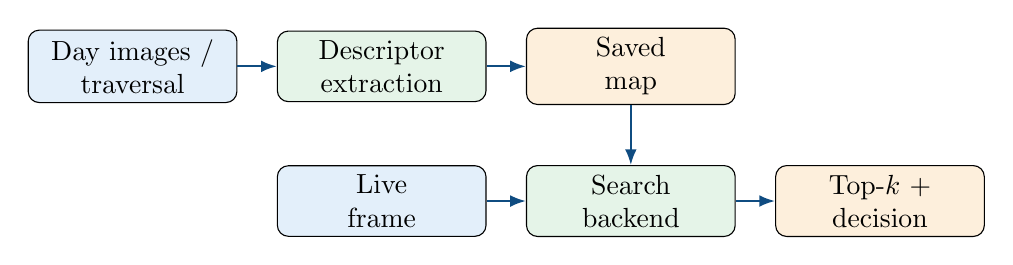
\begin{tikzpicture}[
  node distance=5mm and 5mm,
  box/.style={draw, rounded corners, minimum width=2.65cm, minimum height=0.85cm, align=center, fill=softgray},
  arrow/.style={-{Latex[length=2mm]}, thick, accent}
]
  \node[box, fill=softblue] (map) {Day images /\\traversal};
  \node[box, right=of map, fill=softgreen] (desc) {Descriptor\\extraction};
  \node[box, right=of desc, fill=softorange] (store) {Saved\\map};
  \node[box, below=8mm of desc, fill=softblue] (query) {Live\\frame};
  \node[box, right=of query, fill=softgreen] (search) {Search\\backend};
  \node[box, right=of search, fill=softorange] (result) {Top-$k$ +\\decision};
  \draw[arrow] (map) -- (desc);
  \draw[arrow] (desc) -- (store);
  \draw[arrow] (query) -- (search);
  \draw[arrow] (search) -- (result);
  \draw[arrow] (store.south) -- (search.north);
\end{tikzpicture}
}
\caption{High-level architecture of the live VPR system.}
\end{figure}

\subhead{Our Solution}
We use a \textbf{training-free pipeline} built around strong pre-trained descriptors.
\begin{center}
\resizebox{0.96\linewidth}{!}{%
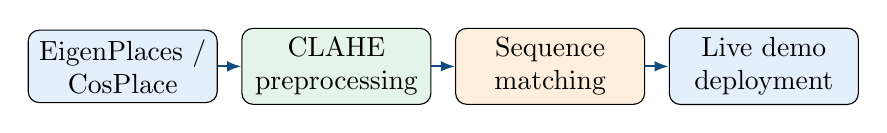
\begin{tikzpicture}[
  node distance=3mm and 3mm,
  tinybox/.style={draw, rounded corners, minimum width=2.4cm, minimum height=0.75cm, align=center, fill=softgray},
  arrow/.style={-{Latex[length=1.8mm]}, thick, accent}
]
  \node[tinybox, fill=softblue] (base) {EigenPlaces /\\CosPlace};
  \node[tinybox, right=of base, fill=softgreen] (clahe) {CLAHE\\preprocessing};
  \node[tinybox, right=of clahe, fill=softorange] (seq) {Sequence\\matching};
  \node[tinybox, right=of seq, fill=softblue] (live) {Live demo\\deployment};
  \draw[arrow] (base) -- (clahe);
  \draw[arrow] (clahe) -- (seq);
  \draw[arrow] (seq) -- (live);
\end{tikzpicture}
}
\end{center}

\begin{itemize}[leftmargin=1.2em,itemsep=0.15em]
  \item \textbf{Baseline}: strong global descriptors.
  \item \textbf{CLAHE}: reduce the day-night appearance gap.
  \item \textbf{Sequence}: improve ranking with temporal context.
  \item \textbf{Live demo}: run from webcam, phone, or robot stream.
\end{itemize}

GardensPoint suggests a \textbf{ranking problem}: the right place is often in the top-$5$, but not always first.

For campus evaluation, we treat relabeling as an \textbf{evaluation fix}, not the main contribution. After manual review, night queries were matched to \textbf{place IDs} rather than one exact day image so same-place, different-view retrievals are credited fairly.

\subhead{Results}
\keyline{The original campus setup was not robust to multiple valid views under a strict image-level evaluation protocol.}

The earlier benchmark was under-crediting correct same-place retrievals. After relabeling the data at the \textbf{place level}, the strongest descriptors improved substantially:

\begin{center}
\small
\begin{tabular}{lccc}
\toprule
\textbf{Model} & \textbf{AUC} & \textbf{R@1} & \textbf{Note} \\
\midrule
CosPlace & 0.627 & 0.969 & strongest top-1 \\
EigenPlaces & \textbf{0.663} & 0.922 & best AUC \\
PatchNetVLAD & 0.641 & 0.938 & strong alternative \\
HDC-DELF & 0.507 & 0.922 & cleaner thresholding \\
\bottomrule
\end{tabular}
\end{center}

\begin{figure}[h]
\centering
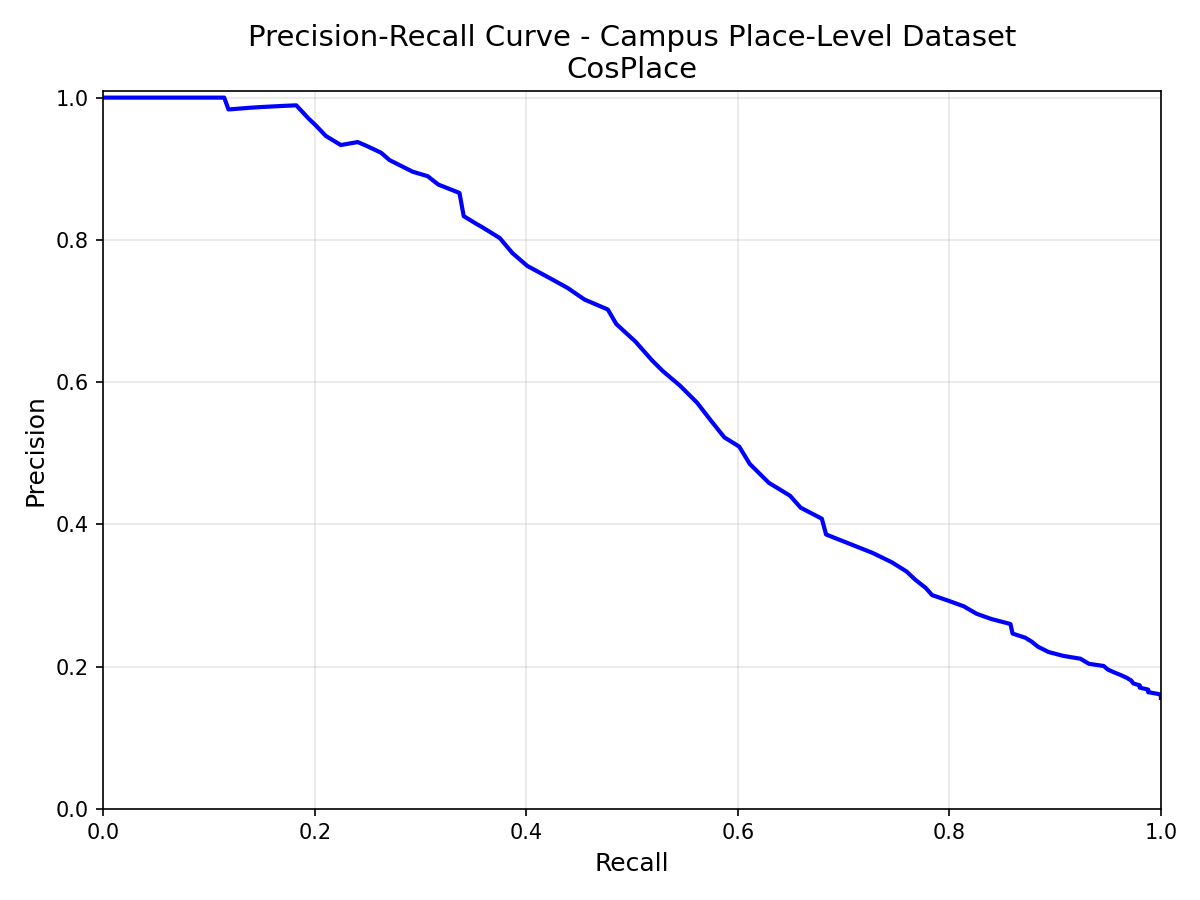
\includegraphics[width=\linewidth,height=4.7cm,keepaspectratio]{../../output_images/campus_place_level_pr_curve.png}
\caption{Place-level PR curve summary on the campus dataset.}
\end{figure}

\begin{figure}[h]
\centering
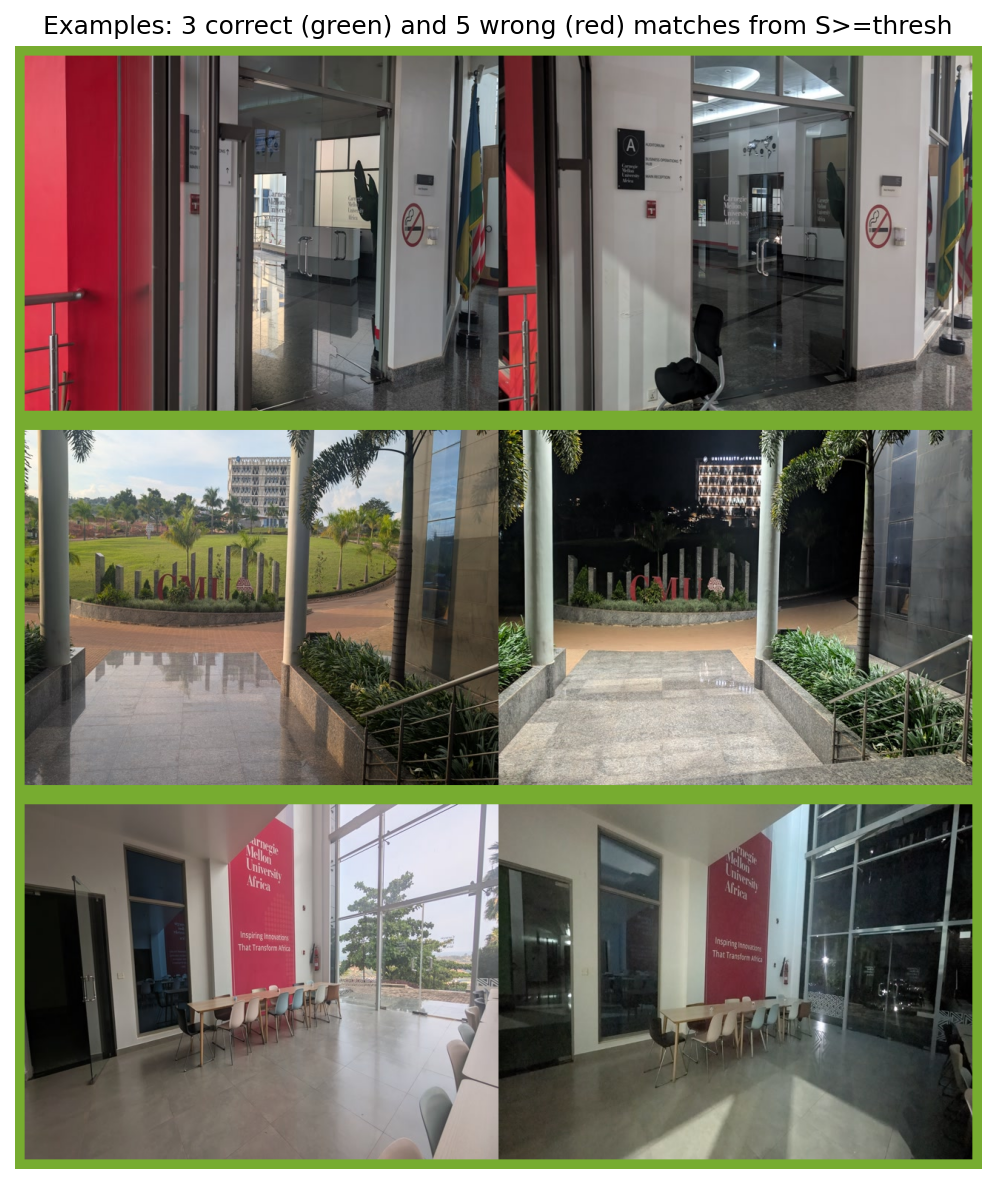
\includegraphics[width=\linewidth,height=3.8cm,keepaspectratio]{../../output_images/campus_place_level_matches_examples.png}
\caption{Qualitative same-place retrieval examples under place-level evaluation.}
\end{figure}

The relabeling changed the story in an important way:
\begin{itemize}[leftmargin=1.2em,itemsep=0.2em]
  \item \textbf{CosPlace}: R@1 improved from \textbf{0.727} to \textbf{0.969}
  \item \textbf{NetVLAD}: R@1 improved from \textbf{0.394} to \textbf{0.891}
  \item \textbf{EigenPlaces}: AUC improved from \textbf{0.443} to \textbf{0.663}
\end{itemize}

This indicates that many earlier “false matches” were not truly wrong places. They were often \textbf{same-place, different-view matches} that the strict labeling protocol did not credit.

\subhead{Future Research}
\begin{itemize}[leftmargin=1.2em,itemsep=0.2em]
  \item Add \textbf{sequence-aware localization} so consecutive frames reinforce one another.
  \item Incorporate \textbf{motion and pose prediction}, for example with a Kalman-filter-style state estimate.
  \item Add a dedicated \textbf{open-set benchmark split} with truly unmatched night queries after place-level review.
  \item Strengthen \textbf{live robot deployment} using the TurboPi camera stream.
\end{itemize}

\subhead{References}
\small
Berton et al., \emph{CosPlace}, CVPR 2022. \quad
Berton et al., \emph{EigenPlaces}, ICCV 2023. \quad
Arandjelovi\'c et al., \emph{NetVLAD}, CVPR 2016. \quad
Milford and Wyeth, \emph{SeqSLAM}, ICRA 2012.

\end{document}
